\chapter{Results}

This chapter discusses the results obtained after training pre-trained language models and baselines. Out of the discussed evaluation metrics, sample-based metrics have been used to evaluate the performance. Visual plots are generated along with the tabular results for better interpretation. 
\\
\\
All the models have been evaluated on both sample-based and label-based metrics. As label-based metrics would fail to address the correlation among different classes \cite{zhang2010multi}, sample-based metrics have been chosen as main evaluation metrics as the stereotypical dataset consists of label dependencies. Hence, the evaluation of fine-tuning and feature-based models using sample-based metrics will be discussed in this section. Evaluation results using label-based metrics can be found in the appendix \ref{appendix}.
\\
\\
Most of the multi-label learning algorithms return real-valued function \cite{zhang2010multi}. These real-valued outputs (mostly probabilities) returned by models must be calibrated against the threshold to decide on the proper or hard label. A popular choice of constant is using 0.5 when the outputs represent posterior probabilities\cite{zhang2010multi}. This thesis uses a threshold of 0.5 to convert the real-valued posterior probabilities into proper labels. Experiments have been performed to calculate the optimal threshold per class using a criterion that maximizes true positive and true negative rates. The results obtained from the two thresholds were calculated. The results have a marginal difference in precision and recall (slightly higher recall for the optimal threshold). The results in this section are obtained by using 0.5 as the threshold. For a fair comparison, all the language and baseline models have been tested on the same test split using both sample-based and label-based metrics. 

\section{Sample-based metrics}
% All the pre-trained models have been used from hugging face library \footnote{\url{https://huggingface.co/transformers/pretrained_models.html}} and experiments were done using PyTorch lightening, hugging face, and ktrain (a wrapper around hugging face and Keras) to fine-tune the language model for the downstream task, i.e., multi-label text classification. Finally, the results BERT and RoBERTa were considered from the Strain library, and for XLNet and GPT-2, the results were considered from using HuggingFace library.
\begin{table}[h!]
\resizebox{\textwidth}{!}{%
\begin{tabular}{@{}llll@{}}
\toprule
Model name  & \multicolumn{3}{c}{Sample Average}  \\ \midrule
\multicolumn{1}{l|}{} & \multicolumn{1}{l|}{precision} & \multicolumn{1}{l|}{recall} & \multicolumn{1}{l|}{f1-score} \\ \cmidrule(l){2-4} 
\multicolumn{1}{l|}{bert-base-uncased} & \multicolumn{1}{l|}{0.8666129898013957} & \multicolumn{1}{l|}{0.8659420289855072} & \multicolumn{1}{l|}{0.8624127750939347} \\ \cmidrule(l){2-4} 
\multicolumn{1}{l|}{roberta-base}      & \multicolumn{1}{l|}{0.9024422973698335} & \multicolumn{1}{l|}{\textbf{0.9013687600644122}} & \multicolumn{1}{l|}{\textbf{0.901207729468599}}  \\ \cmidrule(l){2-4} 
\multicolumn{1}{l|}{gpt2}              & \multicolumn{1}{l|}{0.7897208803005905} & \multicolumn{1}{l|}{0.5940016103059581} & \multicolumn{1}{l|}{0.6582125603864735} \\ \cmidrule(l){2-4} 
\multicolumn{1}{l|}{xlnet-base-cased}  & \multicolumn{1}{l|}{\textbf{0.9118357487922706}} & \multicolumn{1}{l|}{0.7866344605475041} & \multicolumn{1}{l|}{0.8283682232957594} \\ \bottomrule
\end{tabular}%
}
\caption{Sample average precision, recall, f1-score results of Language models with top results highlighted}
\label{tab:sample_avg_LM}
\end{table}
\begin{figure}[h!]
    \centering
    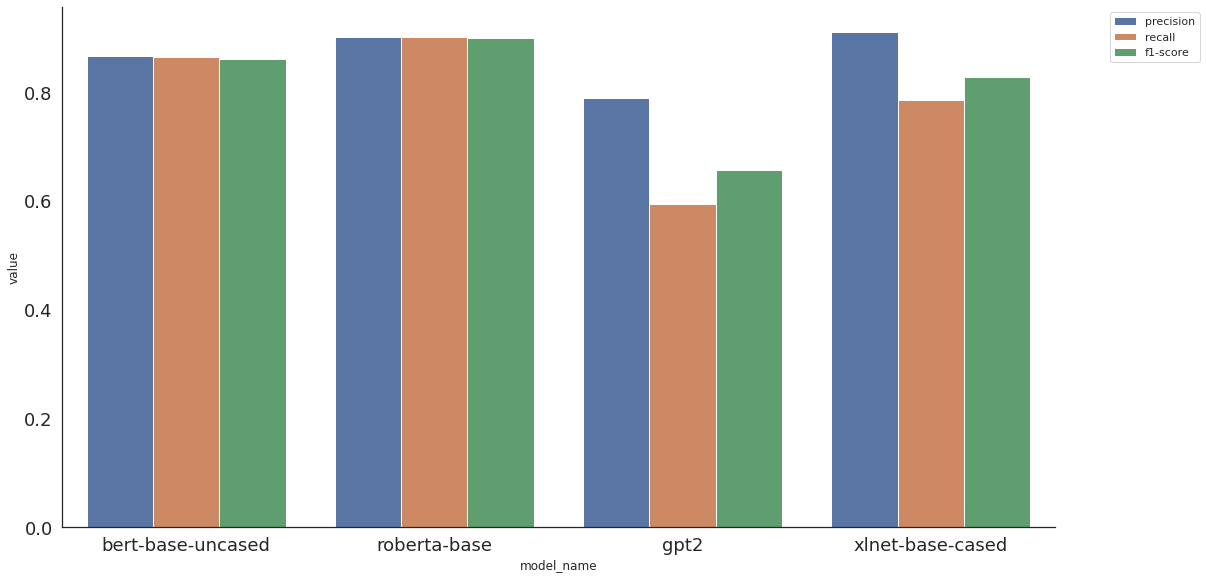
\includegraphics[width=0.8\textwidth]{thesis/figures/Model_wise_prf .png}
    \caption{Sample average precision, recall and f1score grouped model wise }
    \label{fig:model_wise_group_LM}
\end{figure}


\begin{figure}[h!]
    \centering
    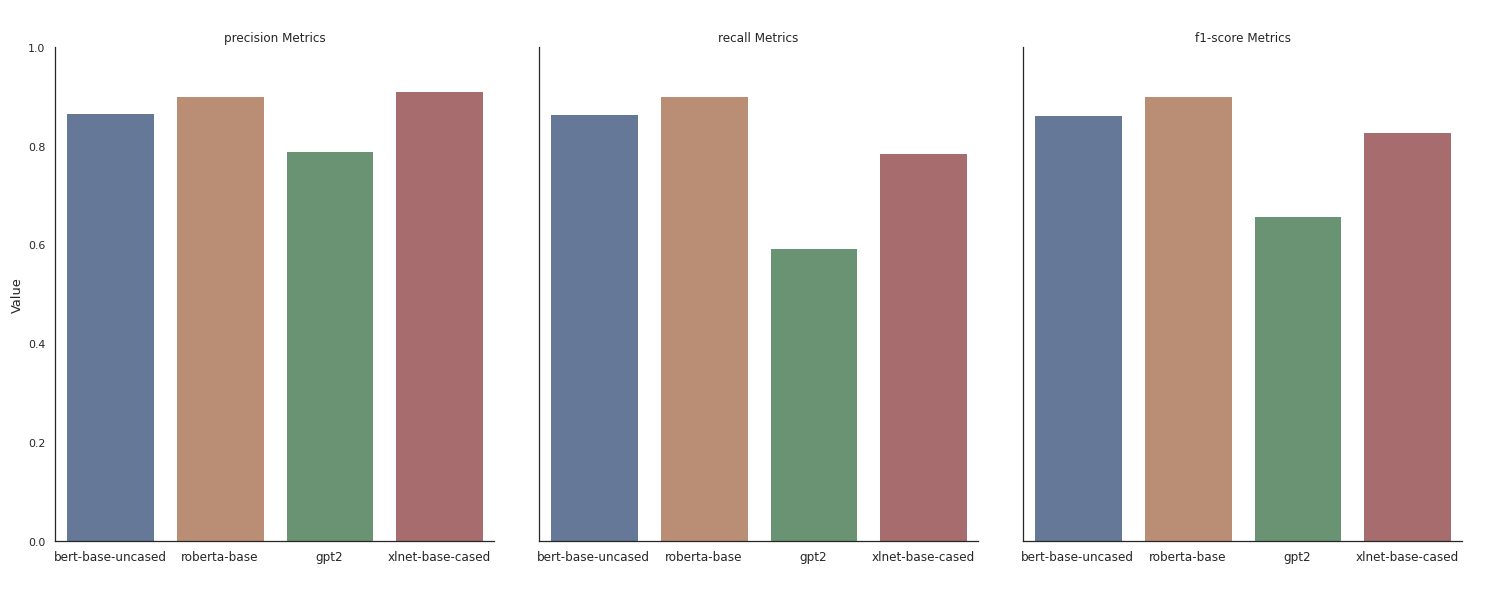
\includegraphics[width=0.8\textwidth]{thesis/figures/labelwise_wise_prf.png}
    \caption{Sample average precision, recall, and f1score grouped label wise }
    \label{fig:label_wise_group_LM}
\end{figure}
Table \ref{tab:sample_avg_LM} shows the results obtained by using sample-based metrics on the test set using language models. As seen in the Table, the XLNet language model has the highest precision compared to another model.  RoBERTa has the highest recall and f1-score when compared to other models. On average, RoBERTa has a stable precision and recall when compared to XLNet. Though the precision of the XLNet model was marginally better by around 1.04\%, the recall score had a drop of 12.7\%  which resulted in an 8.08\% drop in the f1-score compared to RoBERTa. Figure \ref{fig:model_wise_group_LM} shows this property of variance in precision, recall and f1-score for each model. An interesting property is that BERT and RoBERTa language models tend to have low variance in their precision, recall, and f1scores when compared to GPT-2 or XLNet. On average, there is a 4\% difference among precision, recall, and f1-scores between BERT and RoBERTa models. GPT-2 is the worst performing language model, with a very low recall(34.1\% less recall when compared to RoBERTa). Figure \ref{fig:label_wise_group_LM} shows a label wise plot of different language models. On average, precision scores of the different language models seem to be higher when compared to recall. To give an overall rank based on sample average f1-score, RoBERTa is the best performing model, followed by BERT (4.3\% decrease), followed by XLNet (8.08\% decrease), and GPT-2 (26.9\% decrease). 

% \pagebreak

\begin{table}[]
\resizebox{\textwidth}{!}{%
\begin{tabular}{@{}l|l|l|l|@{}}
\toprule
Model name & hamming\_loss       & subset\_accuracy    & hamming\_score/Accuracy   \\ \midrule
bert-base-uncased & 0.07516678168852083  & 0.7137681159420289 & 0.8200483091787394 \\ \cmidrule(l){2-4} 
roberta-base      & \textbf{0.053887738670347365} & \textbf{0.8188405797101449} & \textbf{0.8748322597960254} \\ \cmidrule(l){2-4} 
gpt2       & 0.12928456406717276 & 0.36312399355877617 & 0.5830314009661832      \\ \cmidrule(l){2-4} 
xlnet-base-cased  & 0.07677708764665286  & 0.6203703703703703 & 0.7729468599033793  \\ \bottomrule
\end{tabular}%
}
\caption{Hamming loss, Hamming score, subset accuracy scores of Language models}
\label{tab:hhaa}
\end{table}

\begin{figure}[h!]
    \centering
    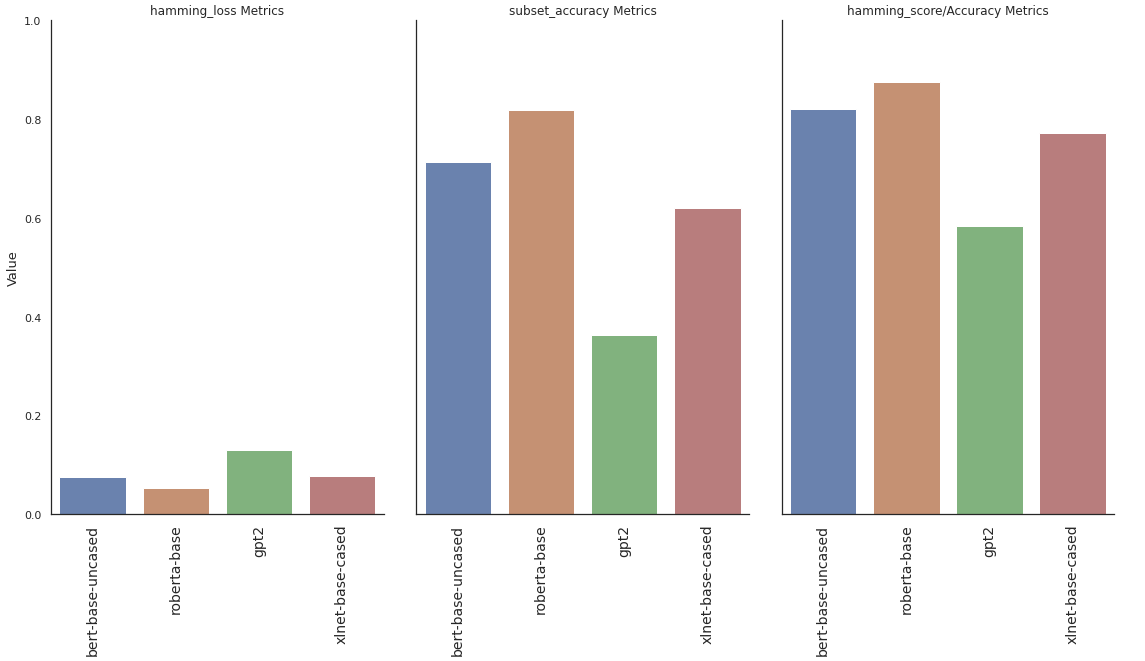
\includegraphics[width=1\textwidth]{thesis/labelwise_hhaa_adjusted.png}
    \caption{Hamming loss, Hamming score, subset accuracy scores of language models grouped label wise }
    \label{fig:hhaa_label_wise_group}
\end{figure}

Table \ref{tab:hhaa} shows the Hamming loss, subset accuracy, Hamming score results obtained on the test set. Hamming loss, as discussed, is the "average per-sample per-class total error" \cite{sokolova2009systematic}. The lower the Hamming loss, the lesser the misprediction. As highlighted in the Table, RoBERTa has the lowest Hamming loss, followed by BERT, which has 39.4\% greater Hamming loss, and XLNet, which has 42.4\% greater Hamming loss when compared to RoBERTa. GPT-2 has the highest Hamming loss. Regarding subset accuracy, which is a harsh measure where the exact match per text is calculated, RoBERTa has the highest subset accuracy score of around 81\%. RoBERTa is followed by BERT, whose subset accuracy is 12.8\% less when compared to RoBERTa followed by XLNet (24.2\% decrease) and GPT-2 (55.6\% decrease). Hamming score (average per-sample partial matches) follows the same pattern where RoBERTa has the highest score, followed by BERT, XLNet, and GPT-2. For RoBERTa, there is a 6.8\% increase in accuracy when considering partial matches (Hamming score) rather than exact matches (subset accuracy); 14.89\% increase for BERT, 24.59\% for XLNet and 60.55\% for GPT-2.
Overall, a clear pattern can be observed from the measures as well as with the visual plot \ref{fig:hhaa_label_wise_group}. Based on Figure  \ref{fig:hhaa_label_wise_group}, RoBERTa is the best performing model, followed by BERT, followed by XLNet, and GPT-2, where RoBERTa outperforms other models.
% \pagebreak

\begin{table}[]
\resizebox{\textwidth}{!}{%
\begin{tabular}{@{}lllll@{}}
\toprule
Model name &
  Text features &
  \multicolumn{3}{c}{Sample average} \\ \midrule
 &
  \multicolumn{1}{l|}{} &
  \multicolumn{1}{l|}{precision} &
  \multicolumn{1}{l|}{recall} &
  \multicolumn{1}{l|}{f1-score} \\ \midrule
\multicolumn{1}{|l|}{\multirow{3}{*}{CNN}} &
  \multicolumn{1}{l|}{Flair embedding model} &
  \multicolumn{1}{l|}{0.474838969} &
  \multicolumn{1}{l|}{0.468196457} &
  \multicolumn{1}{l|}{0.467377885} \\ \cmidrule(l){2-5} 
\multicolumn{1}{|l|}{} &
  \multicolumn{1}{l|}{Glove embedding model} &
  \multicolumn{1}{l|}{0.411567364} &
  \multicolumn{1}{l|}{0.39452496} &
  \multicolumn{1}{l|}{0.399436393} \\ \cmidrule(l){2-5} 
\multicolumn{1}{|l|}{} &
  \multicolumn{1}{l|}{Fasttext embedding model} &
  \multicolumn{1}{l|}{0.407306763} &
  \multicolumn{1}{l|}{0.400563607} &
  \multicolumn{1}{l|}{0.401959206} \\ \midrule
\multicolumn{1}{|l|}{\multirow{2}{*}{MNB}} &
  \multicolumn{1}{l|}{BOW} &
  \multicolumn{1}{l|}{0.738353079} &
  \multicolumn{1}{l|}{0.731280193} &
  \multicolumn{1}{l|}{0.718108913} \\ \cmidrule(l){2-5} 
\multicolumn{1}{|l|}{} &
  \multicolumn{1}{l|}{TF\_IDF} &
  \multicolumn{1}{l|}{0.62003489} &
  \multicolumn{1}{l|}{0.492753623} &
  \multicolumn{1}{l|}{0.534889962} \\ \midrule
\multicolumn{1}{|l|}{SVM} &
  \multicolumn{1}{l|}{Selected featurres} &
  \multicolumn{1}{l|}{0.578166935} &
  \multicolumn{1}{l|}{0.45873591} &
  \multicolumn{1}{l|}{0.4965781} \\ \midrule
\multicolumn{1}{|l|}{\multirow{2}{*}{Decision tree}} &
  \multicolumn{1}{l|}{BOW} &
  \multicolumn{1}{l|}{0.676731079} &
  \multicolumn{1}{l|}{0.676529791} &
  \multicolumn{1}{l|}{0.676596887} \\ \cmidrule(l){2-5} 
\multicolumn{1}{|l|}{} &
  \multicolumn{1}{l|}{TF\_IDF} &
  \multicolumn{1}{l|}{\textbf{0.745169082}} &
  \multicolumn{1}{l|}{\textbf{0.744967794}} &
  \multicolumn{1}{l|}{\textbf{0.74503489}} \\ \midrule
\multicolumn{1}{|l|}{\multirow{2}{*}{KNN}} &
  \multicolumn{1}{l|}{BOW} &
  \multicolumn{1}{l|}{0.542874396} &
  \multicolumn{1}{l|}{0.498590982} &
  \multicolumn{1}{l|}{0.51335212} \\ \cmidrule(l){2-5} 
\multicolumn{1}{|l|}{} &
  \multicolumn{1}{l|}{TF\_IDF} &
  \multicolumn{1}{l|}{0.330515298} &
  \multicolumn{1}{l|}{0.308172303} &
  \multicolumn{1}{l|}{0.315619968} \\ \midrule
\multicolumn{1}{|l|}{\multirow{2}{*}{Random Forest}} &
  \multicolumn{1}{l|}{BOW} &
  \multicolumn{1}{l|}{0.65599839} &
  \multicolumn{1}{l|}{0.569041868} &
  \multicolumn{1}{l|}{0.598027375} \\ \cmidrule(l){2-5} 
\multicolumn{1}{|l|}{} &
  \multicolumn{1}{l|}{TF\_IDF} &
  \multicolumn{1}{l|}{0.736513688} &
  \multicolumn{1}{l|}{0.665458937} &
  \multicolumn{1}{l|}{0.689143854} \\ \midrule
\multicolumn{1}{|l|}{Bi-LSTM} &
  \multicolumn{1}{l|}{Ramdom word embeddings} &
  \multicolumn{1}{l|}{0.452227589} &
  \multicolumn{1}{l|}{0.409219001} &
  \multicolumn{1}{l|}{0.422302737} \\ \bottomrule
\end{tabular}%
}

\caption{Sample average scores of baselines, namely, Convolutional Neural Network (CNN), multinomial Naive Bayes (MNB), Support Vector Machine (SVM), decision trees, k-Nearest Neighbor (KNN), random forests with pre-trained word embedding model, selected features, Term Frequency-Inverse Document Frequency (TF-IDF) and Bag of Words (BOW) as text features}
\label{tab:Sample average scores baselines}
\end{table}

\begin{figure}[h!]
    \centering
    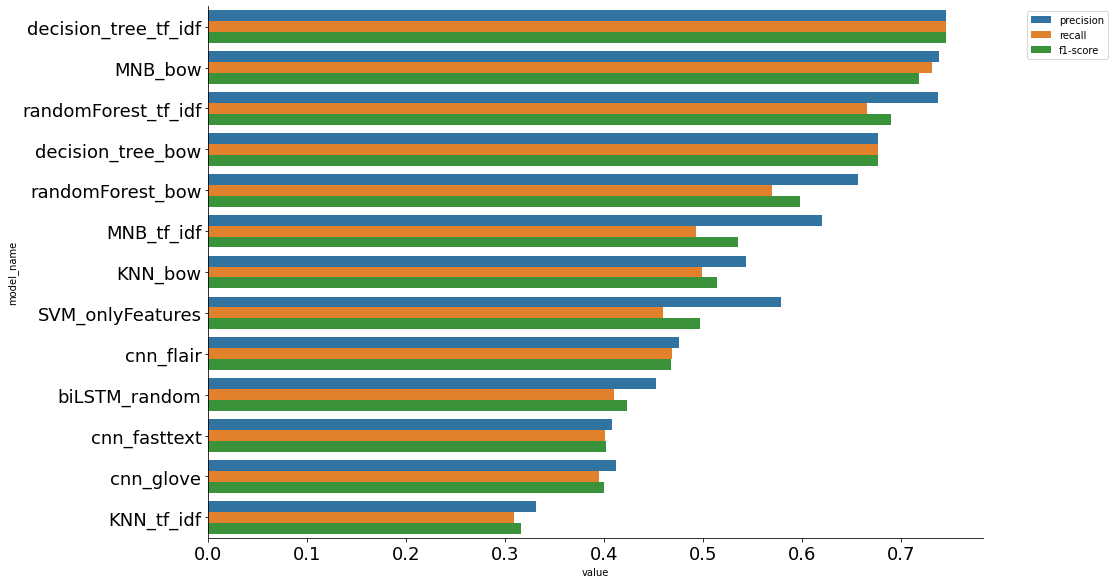
\includegraphics[width=1\textwidth]{thesis/figures/Model_wise_prf.png}
    \caption{Sample average scores of baselines grouped model wise}
    \label{fig:model_wise_group_baselines}
\end{figure}
\pagebreak
\begin{figure}[]
    \centering
    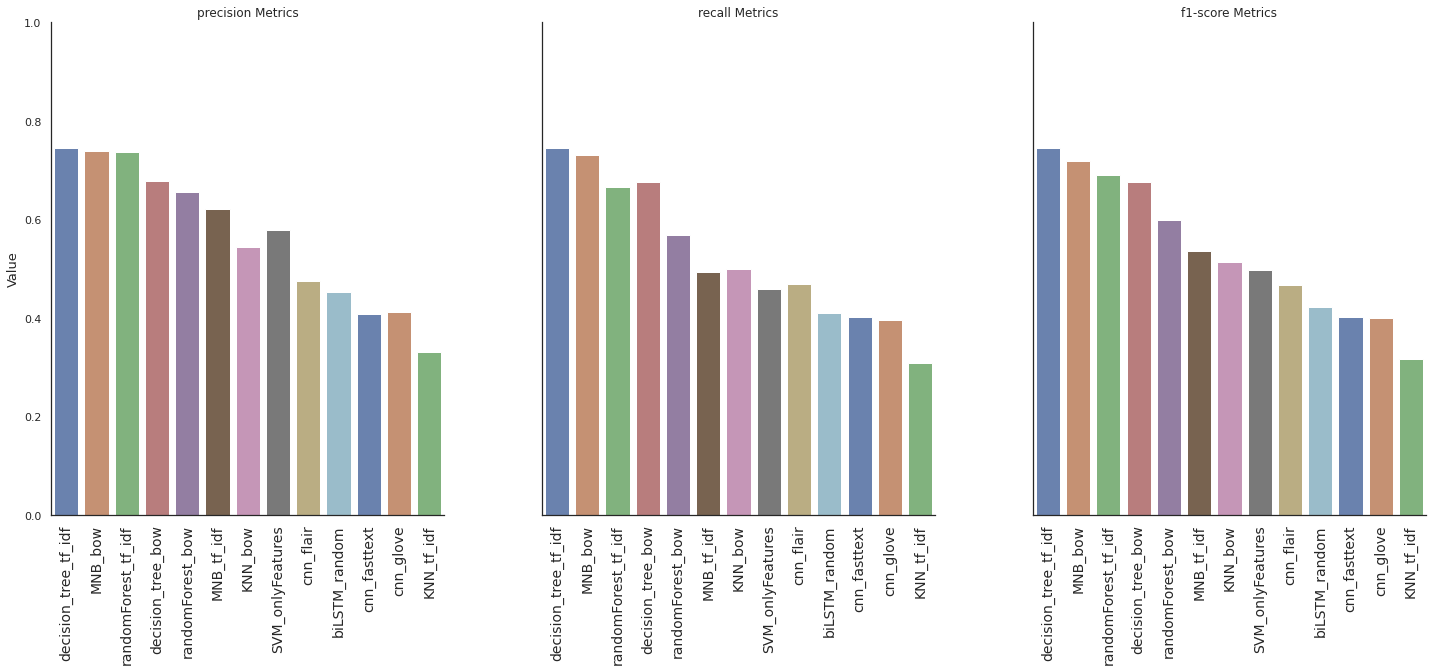
\includegraphics[width=1\textwidth]{thesis/figures/labelwise_wise_prf _baselines.png}
    \caption{Sample average scores of baselines grouped metric wise}
    \label{fig:label_wise_group_baselines}
\end{figure}

Table \ref{tab:Sample average scores baselines} shows the sample average results of the baseline models, which are based on selected text features. Decision tree with Term Frequency-Inverse Document Frequency (TD-IDF) feature has the highest precision. This is followed by multinomial Naive Bayes (MNB) with Bag of Words (BOW) feature with a 0.914\% drop of precision. There is a marginal difference of 0.24\% between the precision scores of random forests with TF-IDF and MNB with BOW feature. On average, the precision scores of deep learning models with pre-trained word embeddings has 40.3\% less precision when compared to decision tree with TF-IDF. Overall precision scores per model can be seen in the Figure \ref{fig:label_wise_group_baselines} where there is a marginal difference in the top three models i.e decision tree with TF-IDF, MNB with  BOW, random forest with TF-IDF. Coming to recall, Decision tree with TF-IDF has the highest recall, followed by MNB with BOW. There is a marginal difference of 1.83\% between recall scores of decision tree with TF-IDF and MNB with BOW. Decision tree with BOW has next highest recall to the MNB with BOW. F1-score of decision tree with TF-IDF has the highest score, followed by MNB with BOW. Overall ranking can be inferred from the Figure \ref{fig:model_wise_group_baselines}; Where the top three are Decision tree with TF-IDF, MNB with BOW and random forests with TF-IDF. Among the deep learning model CNN with flair word embedding has the highest f1-score followed by Bi-directional Long Short-Term Memory Network (biLSTM) with randomly initialized word embeddings. SVM with selected features has 5.8\% higher f1-score when compared to best performing model among deep learning models (CNN with flair word embedding). KNN with TF-IDF is the worst performing model among others.
\pagebreak

\begin{table}[h!]
\resizebox{\textwidth}{!}{%
\begin{tabular}{@{}llrrrr@{}}
\toprule
Model\_name &
  Text features &
  hamming\_loss &
  subset\_accuracy &
  hamming\_score  \\ \midrule
\multicolumn{1}{|l|}{\multirow{3}{*}{CNN}} &
  \multicolumn{1}{l|}{Flair word embedding} &
  \multicolumn{1}{l|}{0.25368069933287324} &
  \multicolumn{1}{l|}{0.3333333333333333} &
  \multicolumn{1}{l|}{0.4270330112721436} \\ \cmidrule(l){2-5} 
\multicolumn{1}{|l|}{} &
  \multicolumn{1}{l|}{Glove word embedding} &
  \multicolumn{1}{l|}{0.27639751552795033} &
  \multicolumn{1}{l|}{0.28140096618357485} &
  \multicolumn{1}{l|}{0.3626207729468618} \\ \cmidrule(l){2-5} 
\multicolumn{1}{|l|}{} &
  \multicolumn{1}{l|}{Fasttext word embedding} &
  \multicolumn{1}{l|}{0.29054520358868186} &
  \multicolumn{1}{l|}{0.26811594202898553} &
  \multicolumn{1}{l|}{0.35874261943102803}  \\ \midrule
\multicolumn{1}{|l|}{\multirow{2}{*}{MNB}} &
  \multicolumn{1}{l|}{Bow} &
  \multicolumn{1}{l|}{\textbf{0.13526570048309178}} &
  \multicolumn{1}{l|}{0.45450885668276975} &
  \multicolumn{1}{l|}{0.648364772640133}  \\ \cmidrule(l){2-5} 
\multicolumn{1}{|l|}{} &
  \multicolumn{1}{l|}{Tf-idf} &
  \multicolumn{1}{l|}{0.15407177363699104} &
  \multicolumn{1}{l|}{0.32286634460547503} &
  \multicolumn{1}{l|}{0.4786298980139564} \\ \midrule
\multicolumn{1}{|l|}{SVM} &
  \multicolumn{1}{l|}{Selected features} &
  \multicolumn{1}{l|}{0.17506326201978376} &
  \multicolumn{1}{l|}{0.2741545893719807} &
  \multicolumn{1}{l|}{0.4379696725711228}  \\ \midrule
\multicolumn{1}{|l|}{\multirow{2}{*}{Decision tree}} &
  \multicolumn{1}{l|}{Bow} &
  \multicolumn{1}{l|}{0.17540832758224062} &
  \multicolumn{1}{l|}{0.4887278582930757} &
  \multicolumn{1}{l|}{0.6139962426194246}  \\ \cmidrule(l){2-5} 
\multicolumn{1}{|l|}{} &
  \multicolumn{1}{l|}{Tf-idf} &
  \multicolumn{1}{l|}{0.13791120312859442} &
  \multicolumn{1}{l|}{\textbf{0.5837359098228664}} &
  \multicolumn{1}{l|}{\textbf{0.6912909286097624}} \\ \midrule
\multicolumn{1}{|l|}{\multirow{2}{*}{KNN}} &
  \multicolumn{1}{l|}{Bow} &
  \multicolumn{1}{l|}{0.20864964343225212} &
  \multicolumn{1}{l|}{0.35829307568438} &
  \multicolumn{1}{l|}{0.46658615136876125}  \\ \cmidrule(l){2-5} 
\multicolumn{1}{|l|}{} &
  \multicolumn{1}{l|}{Tf-idf} &
  \multicolumn{1}{l|}{0.25718886588451806} &
  \multicolumn{1}{l|}{0.2608695652173913} &
  \multicolumn{1}{l|}{0.29985238862050506}  \\ \midrule
\multicolumn{1}{|l|}{\multirow{2}{*}{Random Forest}} &
  \multicolumn{1}{l|}{Bow} &
  \multicolumn{1}{l|}{0.1642512077294686} &
  \multicolumn{1}{l|}{0.36594202898550726} &
  \multicolumn{1}{l|}{0.5303274288781523} & \\ \cmidrule(l){2-5}
\multicolumn{1}{|l|}{} &
  \multicolumn{1}{l|}{Tf-idf} &
  \multicolumn{1}{l|}{0.1376236484932137} &
  \multicolumn{1}{l|}{0.47987117552334946} &
  \multicolumn{1}{l|}{0.6272812667740167} & \\ \midrule
\multicolumn{1}{|l|}{Bi-LSTM} &
  \multicolumn{1}{l|}{Ramdom word embeddings} &
  \multicolumn{1}{l|}{0.25960432482171614} &
  \multicolumn{1}{l|}{0.2713365539452496} &
  \multicolumn{1}{l|}{0.3784219001610322} \\ \bottomrule
\end{tabular}%
}
\caption{Hamming loss, Hamming score, subset accuracy scores of baselines, namely, Convolutional Neural Network (CNN), multinomial Naive Bayes (MNB), Support Vector Machine (SVM), decision trees, k-Nearest Neighbor (KNN), random forests with pre-trained word embedding model, selected features, Term Frequency-Inverse Document Frequency (TD-IDF) and Bag of Words (BOW) as text features}
\label{tab:sample_based_baseline}
\end{table}

\begin{figure}[h!]
    \centering
    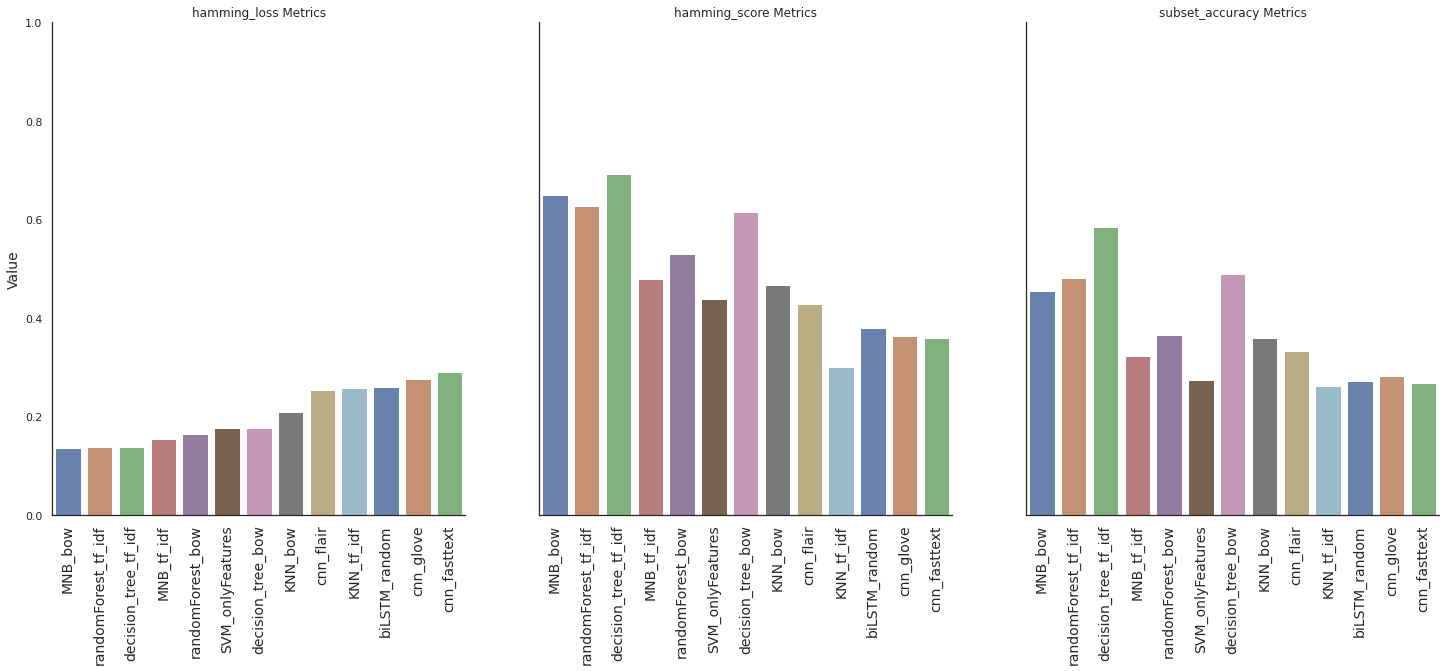
\includegraphics[width=1\textwidth]{thesis/figures/HHAA_final.png}
    \caption{Hamming loss, Hamming score, subset accuracy scores of language models grouped label wise}
    \label{fig:label_wise_hhaa_baselines}
\end{figure}

Table \ref{tab:sample_based_baseline} shows the Hamming loss and accuracy along with subset accuracy. MNB with BOW has the lowest Hamming loss followed by random forests with TF-IDF and decision tree with TF-IDF. Decision tree with TF-IDF has 0.2\% higher loss when compared to random forests with TF-IDF. Overall results among different models can be found in \ref{fig:label_wise_group_baselines}. The Hamming loss of the top three models tends to have negligible differences. A decision tree with TF-IDF features has the highest subset accuracy, followed by a decision tree with BOW features, with a difference of 16.27\%. Random forest with TF-IDF has the next highest subset accuracy. CNN with flair embedding has the highest subset accuracy among deep learning models. SVM with selected features and biLSTM with random word embedding have a negligible difference in their scores (SVM 1.02\% higher).  Coming to Hamming score or accuracy with partial matches, decision tree with TF-IDF features has the highest Hamming score with 15.55\% rise in value when considering partial matches rather than exact match (subset accuracy). MNB with BOW features has the next best Hamming score with 42.65\% increase in accuracy when considering partial matches, followed by random forest with TF-IDF. From the Figure \ref{fig:label_wise_hhaa_baselines} and from the analysis, the best performing model per metric varies. Considering Hamming loss, \acrlong{mnb} with \acrlong{bow} model has a low loss; considering subset accuracy decision tree with TF-IDF, MNB with BOW features and random forest with TF-IDF are the top 3 best performing models. For subset accuracy, again, random forest with TF-IDF,  random forest with TF-IDF, and MNB with BOW features are the best performing models.
